\begin{figure}[H]
    \centering
    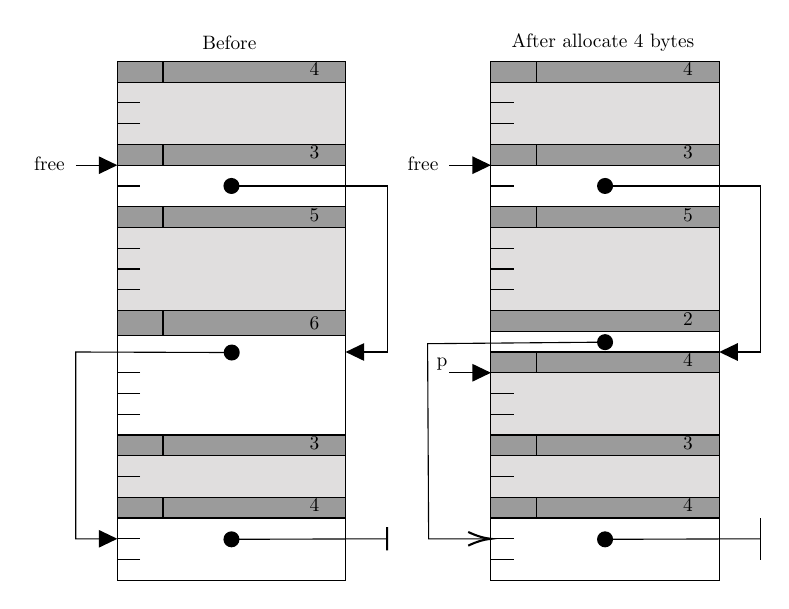
\begin{tikzpicture}[x=0.75pt,y=0.75pt,yscale=-1,xscale=1]
        \draw  [fill={rgb, 255:red, 155; green, 155; blue, 155 }  ,fill opacity=1 ] (100,20) -- (210,20) -- (210,30) -- (100,30) -- cycle ;
        \draw  [fill={rgb, 255:red, 224; green, 222; blue, 222 }  ,fill opacity=1 ] (100,30) -- (210,30) -- (210,60) -- (100,60) -- cycle ;
        \draw    (100,40) -- (111,40) ;
        \draw    (111,50) -- (100,50) ;
        \draw    (122,20) -- (122,30) ;
        \draw  [fill={rgb, 255:red, 155; green, 155; blue, 155 }  ,fill opacity=1 ] (100,60) -- (210,60) -- (210,70) -- (100,70) -- cycle ;
        \draw  [fill={rgb, 255:red, 255; green, 255; blue, 255 }  ,fill opacity=1 ] (100,70) -- (210,70) -- (210,90) -- (100,90) -- cycle ;
        \draw    (100,80) -- (111,80) ;
        \draw    (122,60) -- (122,70) ;
        \draw  [fill={rgb, 255:red, 224; green, 222; blue, 222 }  ,fill opacity=1 ] (100,100) -- (210,100) -- (210,140) -- (100,140) -- cycle ;
        \draw  [fill={rgb, 255:red, 155; green, 155; blue, 155 }  ,fill opacity=1 ] (100,90) -- (210,90) -- (210,100) -- (100,100) -- cycle ;
        \draw    (111,110) -- (100,110) ;
        \draw    (111,120) -- (100,120) ;
        \draw    (111,130) -- (100,130) ;
        \draw    (122,90) -- (122,100) ;
        \draw  [fill={rgb, 255:red, 255; green, 255; blue, 255 }  ,fill opacity=1 ] (100,152) -- (210,152) -- (210,200) -- (100,200) -- cycle ;
        \draw  [fill={rgb, 255:red, 155; green, 155; blue, 155 }  ,fill opacity=1 ] (100,140) -- (210,140) -- (210,152) -- (100,152) -- cycle ;
        \draw    (111,170) -- (100,170) ;
        \draw    (111,180) -- (100,180) ;
        \draw    (122,140) -- (122,152) ;
        \draw    (111,190) -- (100,190) ;
        \draw  [fill={rgb, 255:red, 155; green, 155; blue, 155 }  ,fill opacity=1 ] (100,200) -- (210,200) -- (210,210) -- (100,210) -- cycle ;
        \draw    (122,200) -- (122,210) ;
        \draw  [fill={rgb, 255:red, 224; green, 222; blue, 222 }  ,fill opacity=1 ] (100,210) -- (210,210) -- (210,230) -- (100,230) -- cycle ;
        \draw    (111,220) -- (100,220) ;
        \draw  [fill={rgb, 255:red, 155; green, 155; blue, 155 }  ,fill opacity=1 ] (100,230) -- (210,230) -- (210,240) -- (100,240) -- cycle ;
        \draw  [fill={rgb, 255:red, 255; green, 255; blue, 255 }  ,fill opacity=1 ] (100,240) -- (210,240) -- (210,270) -- (100,270) -- cycle ;
        \draw    (100,250) -- (111,250) ;
        \draw    (111,260) -- (100,260) ;
        \draw    (122,230) -- (122,240) ;
        \draw    (155,80) -- (230,80) -- (230,160) -- (212,160) ;
        \draw [shift={(210,160)}, rotate = 360] [fill={rgb, 255:red, 0; green, 0; blue, 0 }  ][line width=0.75]  [draw opacity=0] (8.93,-4.29) -- (0,0) -- (8.93,4.29) -- cycle    ;
        \draw [shift={(155,80)}, rotate = 0] [color={rgb, 255:red, 0; green, 0; blue, 0 }  ][fill={rgb, 255:red, 0; green, 0; blue, 0 }  ][line width=0.75]      (0, 0) circle [x radius= 3.35, y radius= 3.35]   ;
        \draw    (155.13,160.25) -- (80,160) -- (80,250) -- (98,250) ;
        \draw [shift={(100,250)}, rotate = 180] [fill={rgb, 255:red, 0; green, 0; blue, 0 }  ][line width=0.75]  [draw opacity=0] (8.93,-4.29) -- (0,0) -- (8.93,4.29) -- cycle    ;
        \draw [shift={(155.13,160.25)}, rotate = 180.19] [color={rgb, 255:red, 0; green, 0; blue, 0 }  ][fill={rgb, 255:red, 0; green, 0; blue, 0 }  ][line width=0.75]      (0, 0) circle [x radius= 3.35, y radius= 3.35]   ;
        \draw    (80,70) -- (98,70) ;
        \draw [shift={(100,70)}, rotate = 180] [fill={rgb, 255:red, 0; green, 0; blue, 0 }  ][line width=0.75]  [draw opacity=0] (8.93,-4.29) -- (0,0) -- (8.93,4.29) -- cycle    ;
        \draw    (155,250.25) -- (230,250) ;
        \draw [shift={(230,250)}, rotate = 539.81] [color={rgb, 255:red, 0; green, 0; blue, 0 }  ][line width=0.75]    (0,5.59) -- (0,-5.59)   ;
        \draw [shift={(155,250.25)}, rotate = 359.81] [color={rgb, 255:red, 0; green, 0; blue, 0 }  ][fill={rgb, 255:red, 0; green, 0; blue, 0 }  ][line width=0.75]      (0, 0) circle [x radius= 3.35, y radius= 3.35]   ;
        \draw  [fill={rgb, 255:red, 155; green, 155; blue, 155 }  ,fill opacity=1 ] (280,20) -- (390,20) -- (390,30) -- (280,30) -- cycle ;
        \draw  [fill={rgb, 255:red, 224; green, 222; blue, 222 }  ,fill opacity=1 ] (280,30) -- (390,30) -- (390,60) -- (280,60) -- cycle ;
        \draw    (280,40) -- (291,40) ;
        \draw    (291,50) -- (280,50) ;
        \draw    (302,20) -- (302,30) ;
        \draw  [fill={rgb, 255:red, 155; green, 155; blue, 155 }  ,fill opacity=1 ] (280,60) -- (390,60) -- (390,70) -- (280,70) -- cycle ;
        \draw  [fill={rgb, 255:red, 255; green, 255; blue, 255 }  ,fill opacity=1 ] (280,70) -- (390,70) -- (390,90) -- (280,90) -- cycle ;
        \draw    (280,80) -- (291,80) ;
        \draw    (302,60) -- (302,70) ;
        \draw  [fill={rgb, 255:red, 224; green, 222; blue, 222 }  ,fill opacity=1 ] (280,100) -- (390,100) -- (390,140) -- (280,140) -- cycle ;
        \draw  [fill={rgb, 255:red, 155; green, 155; blue, 155 }  ,fill opacity=1 ] (280,90) -- (390,90) -- (390,100) -- (280,100) -- cycle ;
        \draw    (291,110) -- (280,110) ;
        \draw    (291,120) -- (280,120) ;
        \draw    (291,130) -- (280,130) ;
        \draw    (302,90) -- (302,100) ;
        \draw  [fill={rgb, 255:red, 255; green, 255; blue, 255 }  ,fill opacity=1 ] (280,150) -- (390,150) -- (390,200) -- (280,200) -- cycle ;
        \draw  [fill={rgb, 255:red, 155; green, 155; blue, 155 }  ,fill opacity=1 ] (280,140) -- (390,140) -- (390,150) -- (280,150) -- cycle ;
        \draw  [fill={rgb, 255:red, 155; green, 155; blue, 155 }  ,fill opacity=1 ] (280,200) -- (390,200) -- (390,210) -- (280,210) -- cycle ;
        \draw    (302,200) -- (302,210) ;
        \draw  [fill={rgb, 255:red, 224; green, 222; blue, 222 }  ,fill opacity=1 ] (280,210) -- (390,210) -- (390,230) -- (280,230) -- cycle ;
        \draw    (291,220) -- (280,220) ;
        \draw  [fill={rgb, 255:red, 155; green, 155; blue, 155 }  ,fill opacity=1 ] (280,230) -- (390,230) -- (390,240) -- (280,240) -- cycle ;
        \draw  [fill={rgb, 255:red, 255; green, 255; blue, 255 }  ,fill opacity=1 ] (280,240) -- (390,240) -- (390,270) -- (280,270) -- cycle ;
        \draw    (280,250) -- (291,250) ;
        \draw    (291,260) -- (280,260) ;
        \draw    (302,230) -- (302,240) ;
        \draw    (335,80) -- (410,80) -- (410,160) -- (392,160) ;
        \draw [shift={(390,160)}, rotate = 360] [fill={rgb, 255:red, 0; green, 0; blue, 0 }  ][line width=0.75]  [draw opacity=0] (8.93,-4.29) -- (0,0) -- (8.93,4.29) -- cycle    ;
        \draw [shift={(335,80)}, rotate = 0] [color={rgb, 255:red, 0; green, 0; blue, 0 }  ][fill={rgb, 255:red, 0; green, 0; blue, 0 }  ][line width=0.75]      (0, 0) circle [x radius= 3.35, y radius= 3.35]   ;
        \draw    (260,70) -- (278,70) ;
        \draw [shift={(280,70)}, rotate = 180] [fill={rgb, 255:red, 0; green, 0; blue, 0 }  ][line width=0.75]  [draw opacity=0] (8.93,-4.29) -- (0,0) -- (8.93,4.29) -- cycle    ;
        \draw    (335,250.25) -- (410,250) ;
        \draw [shift={(335,250.25)}, rotate = 359.81] [color={rgb, 255:red, 0; green, 0; blue, 0 }  ][fill={rgb, 255:red, 0; green, 0; blue, 0 }  ][line width=0.75]      (0, 0) circle [x radius= 3.35, y radius= 3.35]   ;
        \draw    (410,240) -- (410,260) ;
        \draw  [fill={rgb, 255:red, 155; green, 155; blue, 155 }  ,fill opacity=1 ] (280,160) -- (390,160) -- (390,170) -- (280,170) -- cycle ;
        \draw  [fill={rgb, 255:red, 224; green, 222; blue, 222 }  ,fill opacity=1 ] (280,170) -- (390,170) -- (390,200) -- (280,200) -- cycle ;
        \draw    (280,180) -- (291,180) ; 
        \draw    (291,190) -- (280,190) ;
        \draw    (302,160) -- (302,170) ; 
        \draw    (260,170) -- (278,170) ;
        \draw [shift={(280,170)}, rotate = 180] [fill={rgb, 255:red, 0; green, 0; blue, 0 }  ][line width=0.75]  [draw opacity=0] (8.93,-4.29) -- (0,0) -- (8.93,4.29) -- cycle    ;
        \draw    (335,155.25) -- (249.5,156) -- (250,250) -- (278,250) ;
        \draw [shift={(280,250)}, rotate = 180] [color={rgb, 255:red, 0; green, 0; blue, 0 }  ][line width=0.75]    (10.93,-3.29) .. controls (6.95,-1.4) and (3.31,-0.3) .. (0,0) .. controls (3.31,0.3) and (6.95,1.4) .. (10.93,3.29)   ;
        \draw [shift={(335,155.25)}, rotate = 179.5] [color={rgb, 255:red, 0; green, 0; blue, 0 }  ][fill={rgb, 255:red, 0; green, 0; blue, 0 }  ][line width=0.75]      (0, 0) circle [x radius= 3.35, y radius= 3.35]   ;
        \draw (195,24) node [scale=0.7] [align=left] {4};
        \draw (195,64) node [scale=0.7] [align=left] {3};
        \draw (195,94) node [scale=0.7] [align=left] {5};
        \draw (195,146) node [scale=0.7] [align=left] {6};
        \draw (195,204) node [scale=0.7] [align=left] {3};
        \draw (195,234) node [scale=0.7] [align=left] {4};
        \draw (67.33,69.33) node [scale=0.7] [align=left] {free};
        \draw (375,24) node [scale=0.7] [align=left] {4};
        \draw (375,64) node [scale=0.7] [align=left] {3};
        \draw (375,94) node [scale=0.7] [align=left] {5};
        \draw (375,144) node [scale=0.7] [align=left] {2};
        \draw (375,204) node [scale=0.7] [align=left] {3};
        \draw (375,234) node [scale=0.7] [align=left] {4};
        \draw (247.33,69.33) node [scale=0.7] [align=left] {free};
        \draw (375,164) node [scale=0.7] [align=left] {4};
        \draw (256.5,166) node [scale=0.7] [align=left] {p};
        \draw (154,11) node [scale=0.7] [align=left] {Before};
        \draw (334,11) node [scale=0.7] [align=left] {After allocate 4 bytes};
    \end{tikzpicture}
    \caption{First-fit allocation policy}
    \label{fig:memman}
\end{figure}